\par Para este experimento realizamos las mediciones sobre una red WiFi laboral durante una hora.

\subsubsection{Fuente $S$}

\par Vemos a continuación las m\'etricas de la fuente $S$ propuesta, modelada con los resultados del experimento: \\

\begin{tabular}{ | c | c | c |}
    \hline
    Mensaje & Probabilidad & Información [bits] \\
    \hline
    \textit{Unicast} & 0.464 & 1.109 \\
    \hline
    \textit{Broadcast} & 0.536 & 0.898 \\
    \hline
\end{tabular} \\

\par Entropía de la fuente: 0.996 bits. Entropía máxima: 1 bit.

\par Podemos observar que los dos tipos de paquetes son casi equiprobables, por lo que la entropía es muy cercana a la máxima.

\par Un resultado llamativo es que m\'as de la mitad de los paquetes hayan sido env\'iados como \textit{broadcast}.
Por tal motivo decidimos analizar en mayor profundidad los paquetes enviados como \textit{broadcast}.

\par En la figura \ref{Tipos de paquetes} podemos ver los resultados de evaluar los diversos tipos de los paquetes \textit{broadcast}.

\begin{figure}[ht]
    \centering
    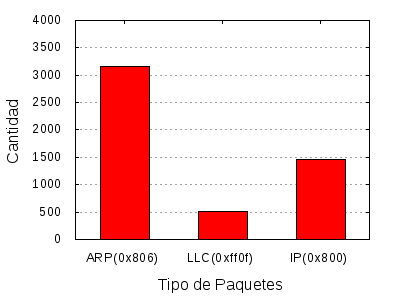
\includegraphics[width=0.45\textwidth]{figuras/experimento2-tipos-paquetes.png}
    \caption{Tipos de paquetes broadcast en el experimento 2.}\label{Tipos de paquetes}
\end{figure}

Como podemos observar en la figura \ref{Tipos de paquetes}, la mayor cantidad de paquetes son de tipo ARP. Podemos notar una pequeña cantidad de paquetes con tipo LLC (Logical Link Control). Éste es propio del estándar IEEE 802.2 que define el control de enlace l\'ogico para redes de \'area local en el modelo OSI. Estos dos tipos de paquetes son utilizados por protocolos de control y su funcionamiento requiere transmisión \textit{broadcast}. Lo llamativo aqu\'i es la gran cantidad de paquetes \textit{broadcast} de tipo IP.

Para mejor comprender esto, graficamos la cantidad de paquetes de este tipo enviados por IP de origen, como se puede ver en la figura \ref{Sources de paquetes IP broadcast}.

\begin{figure*}[ht]
    \centering
    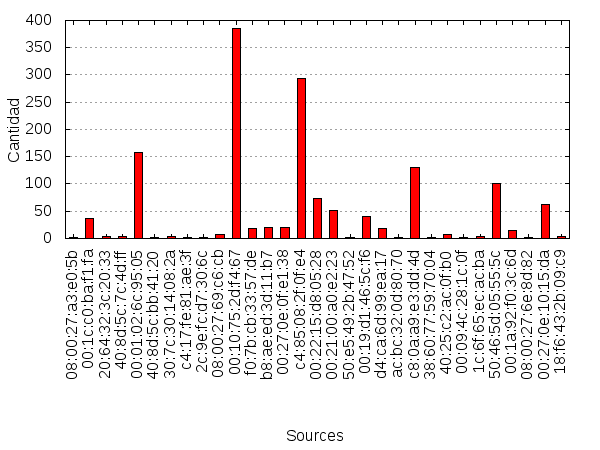
\includegraphics[scale=0.7]{figuras/experimento2-ips-origen.png}
    \caption{MAC addresses de los \textit{sources} de paquetes IP broadcast.}\label{Sources de paquetes IP broadcast}
\end{figure*}

Observemos los tres primeros \textit{sources} que sobresalen del resto en cuanto a cantidad de paquetes enviados. Éstos son los nodos cuyas MAC addresses son: 00:10:75:2d:f4:67 (386 paquetes), c4:85:08:2f:0f:e4 (294 paquetes) y 00:01:02:6c:95:05 (157 paquetes).
Analizando los paquetes de tipo IP que provenían de estos nodos en modo \textit{broadcast}, encontramos que emitían los siguientes mensajes:

\begin{itemize}
	\item 00:10:75:2d:f4:67	: Hello there. I am at 192.168.1.120. Time is 1474050708 and I am hungry.Hostname: backupdyd.seagateshare.com \\
		Notamos que se trata de un software de backup que podr\'ia estar notificando a todos los nodos sus datos para posteriores procesos.
            \item c4:85:08:2f:0f:e4	: De este \textit{source} no pudimos obtener mucha informaci\'on como para poder determinar el propósito de los paquetes \textit{broadcast}.
	\item 00:01:02:6c:95:0: 9016 3 ipp://192.168.1.150:631/printers/HP-LaserJet-P1006 "" "HP LaserJet P1006" "HP LaserJet P1006 Foomatic/foo2xqx (recommended)" job-shee    ts=none,none lease-duration=300 \\
		Se trata de mensajes emitidos por impresoras que eventualmente podr\'ian querer informar sus status a todos los nodos.
\end{itemize}

Por lo tanto, concluimos que se trata de paquetes de control, no de la red en sí misma, sino de protocolos propios de ciertos nodos.

\subsubsection{Estructura de la red en base a los paquetes ARP}

\par En la figura \ref{ARPlaburo} se puede ver el grafo de la red subyacente de mensajes ARP.

\begin{figure*}[ht]
    \centering
    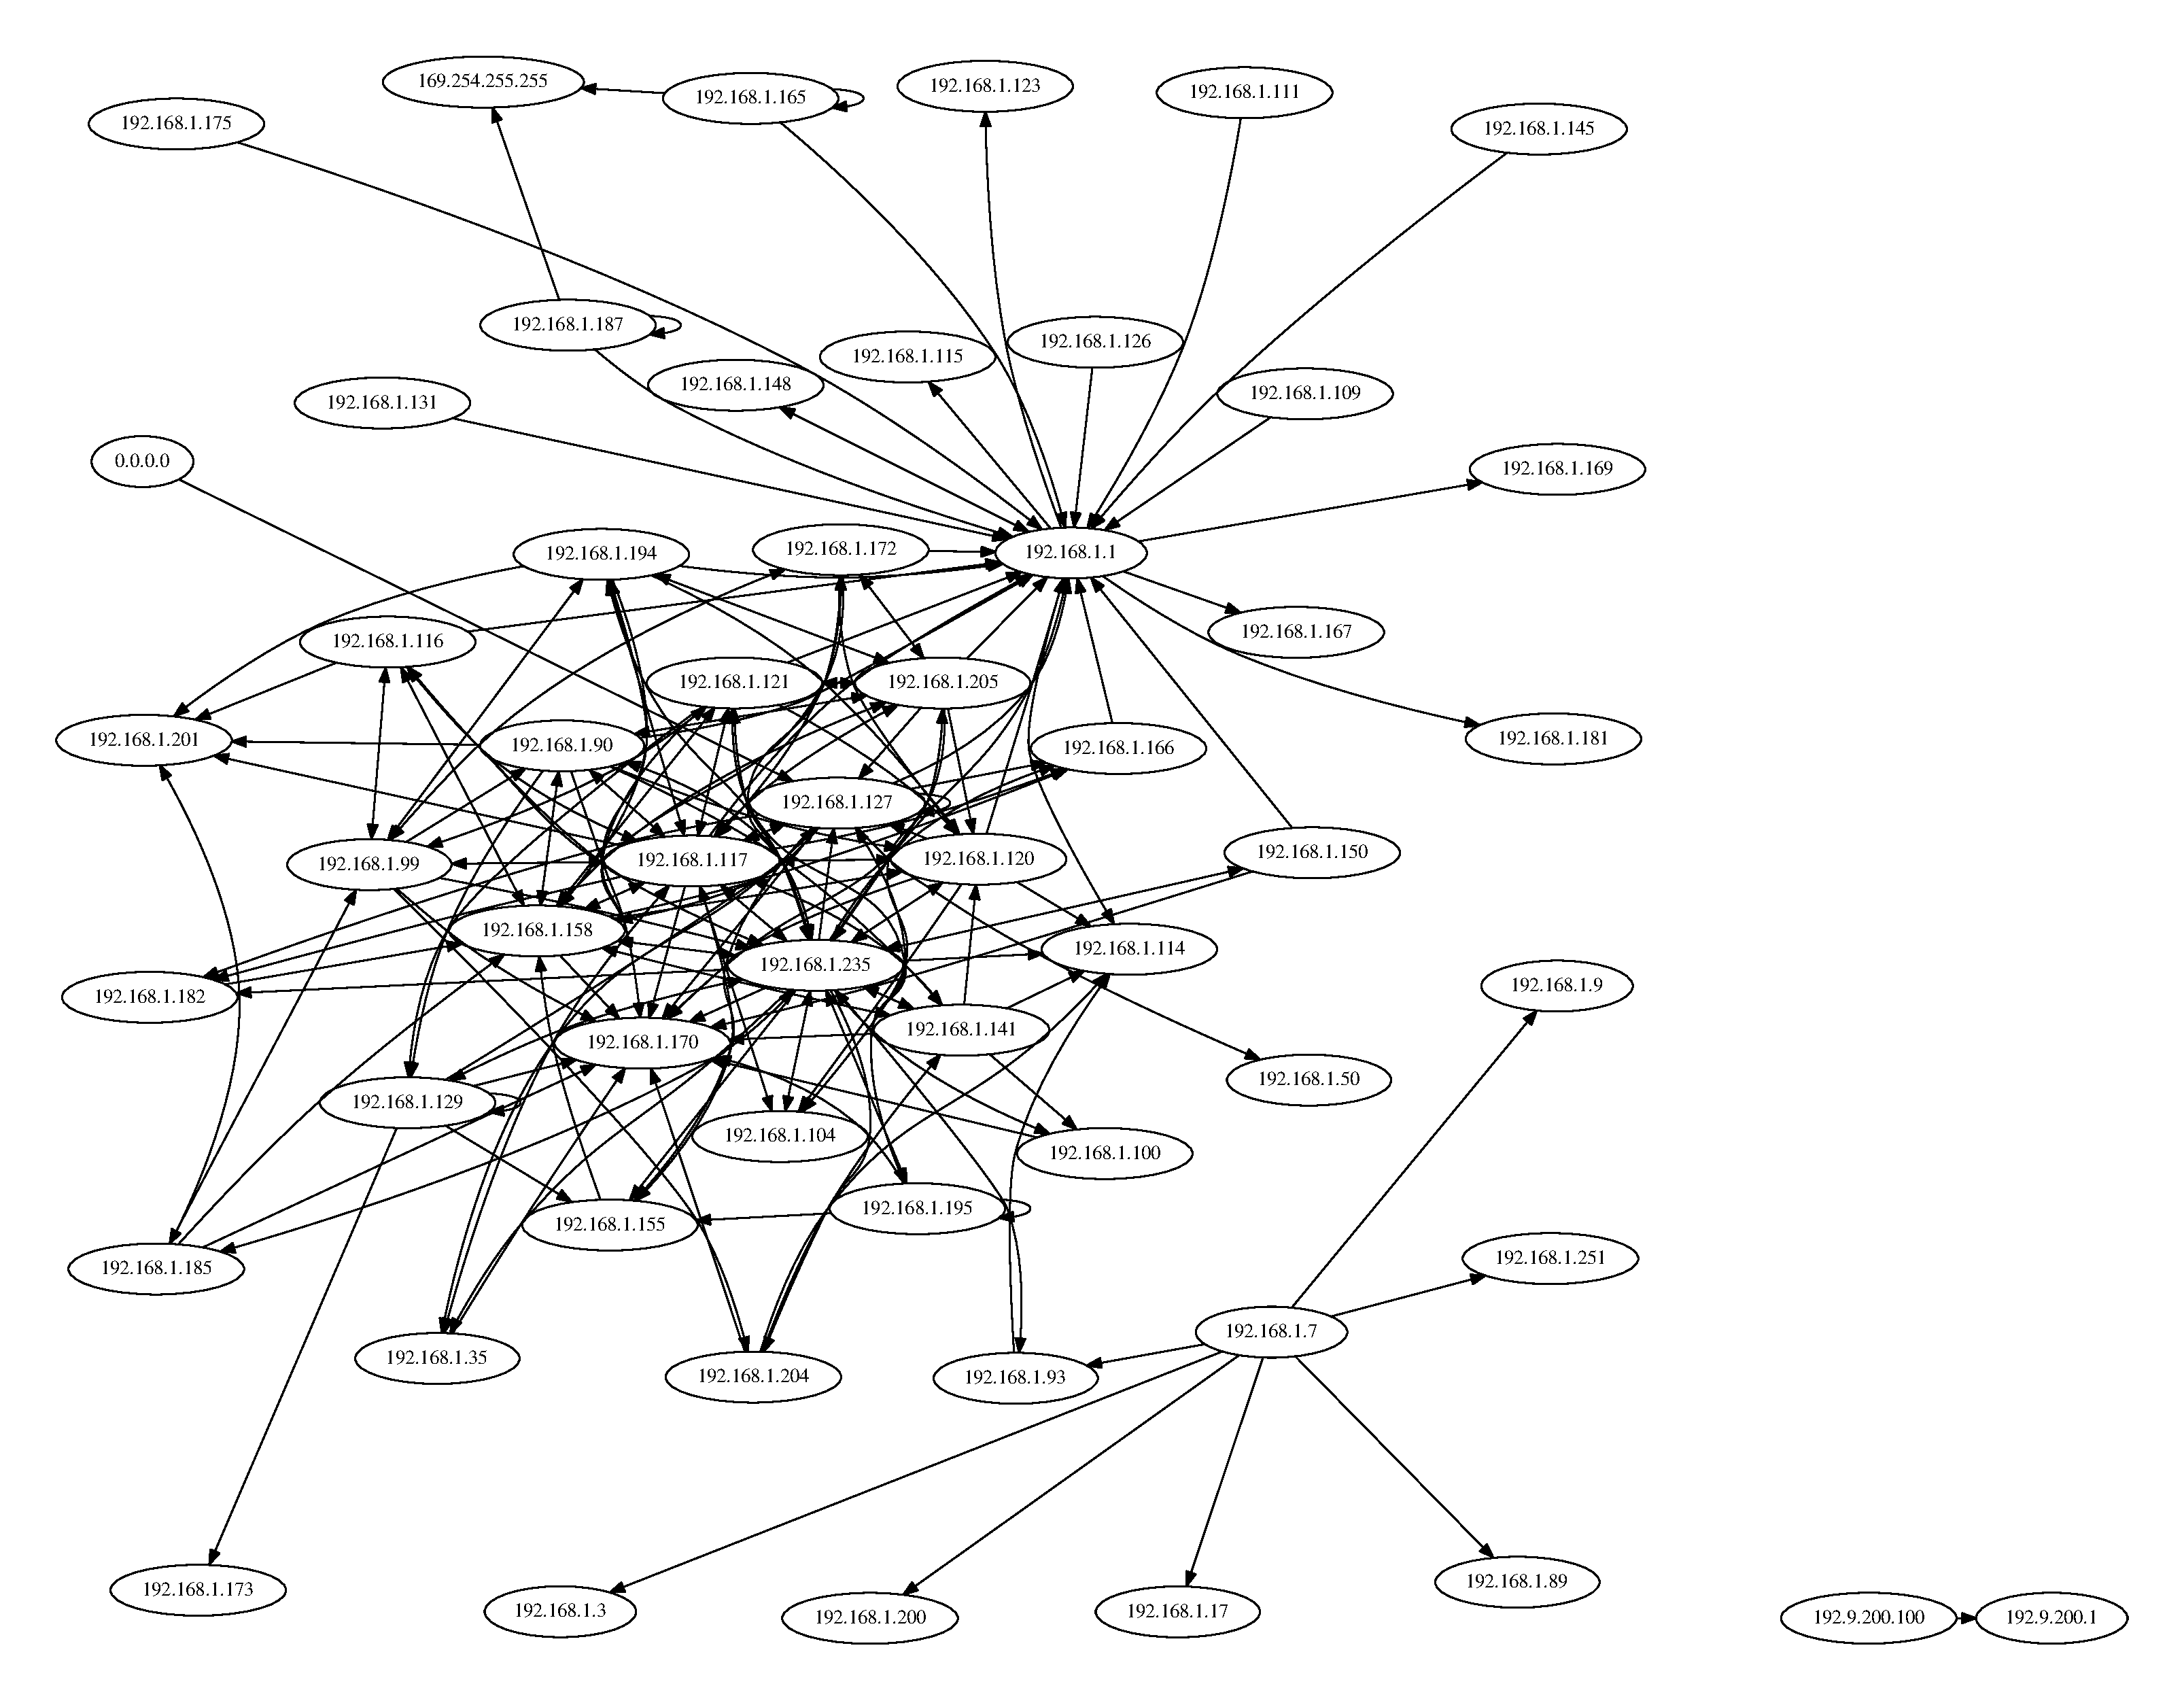
\includegraphics[width=0.9\textwidth]{figuras/laburo_grafo.pdf}
    \caption{Grafo de la red subyacente de mensajes ARP en el experimento 2.}\label{ARPlaburo}
\end{figure*}

\par Las direcciones IP de la red son de la forma 192.168.1.X, con ciertas excepciones: se observa la dirección 0.0.0.0 y la 169.254.255.255, ambas detalladas en el experimento previo; vemos dos nodos con las direcciones 192.9.200.100 y 192.9.200.1.
Adicionalmente, éstos son los únicos dos nodos que no están conectados al resto de la red.
Este comportamiento es anómalo, por lo que creemos que son IPs con un uso particular, específico a la red, ya que no parecen ser reservadas.

\par En el grafo se destaca claramente un nodo, el 192.168.1.1, cuyo comportamiento es consistente con lo esperado de un router\footnote{Es común que los routers ocupen la última o primera, como en este caso, dirección de la red.}.
Luego vemos un grupo de vertices con un muy alto grado de entrada y salida; sin embargo, no parecen actuar como Default Gateways.

\subsubsection{Fuente $S_1$}

\par En la tabla \ref{tab2SinRSinA} podemos ver la información de ciertos mensajes de la fuente $S_1$, sin paquetes repetidos y tomando sólo el \textit{Sender's Protocol Address} de los paquetes.

\par La entropía de la fuente es de 4.61 bits, siendo la máxima 32 bits. 

\begin{table}[t]
    \centering
    \begin{tabular}{ | c | c | c | l |}
        \hline
        Mensaje & Información [bits] & Distinguido?\\
        \hline
192.168.1.1 & 4.86 & No \\
\hline
192.168.1.194 & 4.50 & Sí \\
\hline
192.168.1.127 & 4.50 & Sí \\
\hline
192.168.1.90 & 4.34 & Sí \\
\hline
192.168.1.99 & 4.34 & Sí \\
\hline
192.168.1.121 & 4.34 & Sí \\
\hline
192.168.1.158 & 4.21 & Sí \\
\hline
192.168.1.205 & 4.08 & Sí \\
\hline
192.168.1.117 & 3.34 & Sí \\
\hline
192.168.1.235 & 2.96 & Sí \\
\hline
    \end{tabular} 
    \caption{Información de los nodos de la fuente $S_1$ en el experimento 2, sin tomar paquetes repetidos y considerando como mensaje la ocurrencia de una IP en el campo \textit{Sender's Protocol Address} de un paquete ARP \textit{who-has}.}
    \label{tab2SinRSinA}
\end{table} 

\par El resultado es el opuesto al esperado: los nodos distinguidos son los pertenecientes al grupo de vértices mencionado con alto grado de interconexión pero sin comportamiento de router, mientras que el nodo efectivamente identificado como Default Gateway no es distinguido.

\par En la tabla \ref{tab2A} podemos ver la información de ciertos mensajes de la fuente $S_1$, sin paquetes repetidos y tomando tanto el \textit{Sender's Protocol Address} como el \textit{Target Protocol Address} de los paquetes.

\begin{table}[t]
    \centering
    \begin{tabular}{ | c | c | c | l |}
        \hline
        Mensaje & Información [bits] & Distinguido?\\
\hline
192.168.1.194 & 4.86 & Sí \\
\hline
192.168.1.90 & 4.76 & Sí \\
\hline
192.168.1.99 & 4.67 & Sí \\
\hline
192.168.1.120 & 4.67 & Sí \\
\hline
192.168.1.121 & 4.67 & Sí \\
\hline
192.168.1.127 & 4.67 & Sí \\
\hline
192.168.1.170 & 4.50 & Sí \\
\hline
192.168.1.205 & 4.34 & Sí \\
\hline
192.168.1.158 & 4.08 & Sí \\
\hline
192.168.1.1 & 3.86 & Sí \\
\hline
192.168.1.117 & 3.58 & Sí \\
\hline
192.168.1.235 & 3.24 & Sí \\
\hline
    \end{tabular} 
    \caption{Información de los nodos de la fuente $S_1$ en el experimento 2, sin tomar paquetes repetidos y considerando como mensaje la ocurrencia de una IP tanto en el campo \textit{Sender's Protocol Address} como en el \textit{Target Protocol Address} de un paquete ARP \textit{who-has}.}
    \label{tab2A}
\end{table} 

\par La entropía de la fuente es de 4.93 bits, siendo la máxima 32 bits. 

\par Nuevamente se presentan los falsos positivos, pero el nodo que identificamos como router se considera ahora distinguido.
